% Ch3 Algorithm
\chapter{路徑規劃與控制法則}
\label{c:obstacle_avoidance}

本論文之路徑規劃係利用目標點位置與車輛位置之間的相對關係,以及車輛本身相對於地面的方位角$\psi$,
計算出目標點相對於車輛的角度$\Theta_t$與最短距離$\sigma_t$,並使用這些參數將機器人依序導引至目標點,
同時在導航的過程中必須要避開障礙物,如圖~\ref{f:path_planning}所示。
\begin{figure}
	\centering
	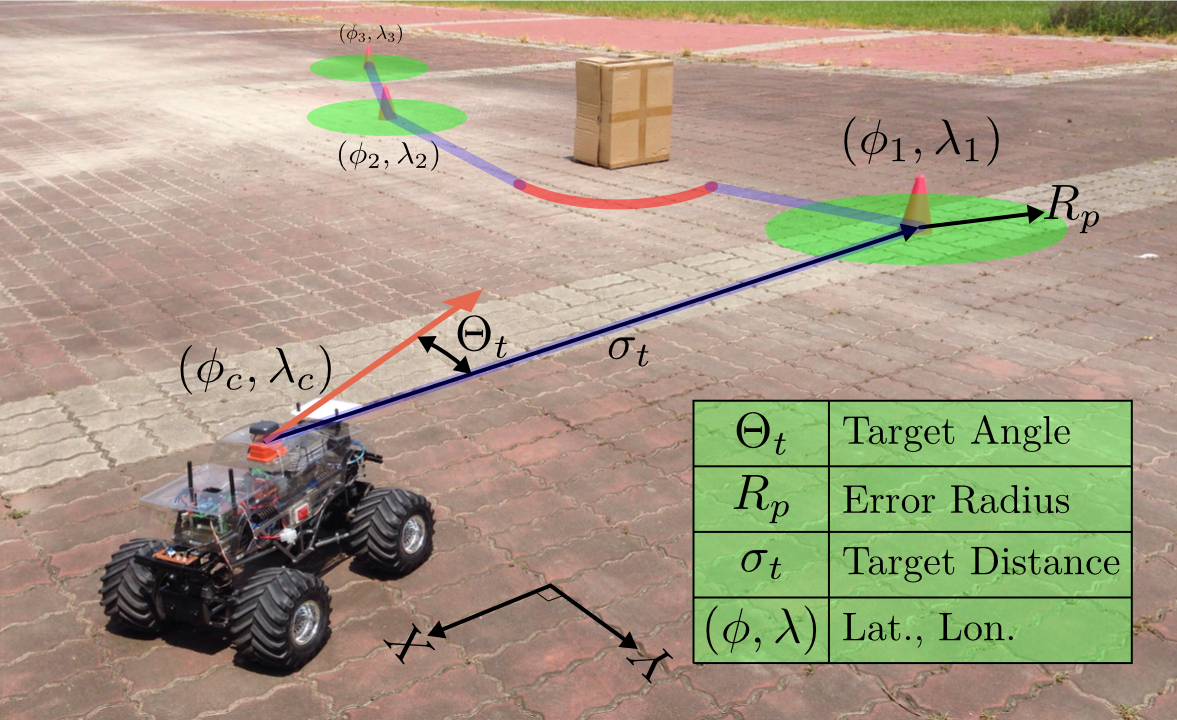
\includegraphics[width=\textwidth]{figures/algorithm/pathplanning}
	\caption{路徑規劃目標}
	\label{f:path_planning}
\end{figure}

由於位置單位為經緯度,\ref{sec:target}節介紹了由經緯度計算$\Theta_t$與$\sigma_t$
之方法。而利用$\Theta_t$、$\sigma_t$與光學雷達所得到的環境資訊,
本論文基於VFH+~\cite{Ulrich:1998:VFHPlus}開發出一避障演算法計算出前進方向,
以避開障礙物,\ref{sec:vfhplus}節介紹其架構。

由於位置量測存在誤差,因此當目標點與車輛的距離$\sigma_t$小於一設定的距離$R_p$時,
便判定車輛已到達該目標點,並開始導航至下一目標點。導航的完整流程圖如圖~\ref{f:navigation_flow}所示:
\begin{figure}[h!]
	\centering
	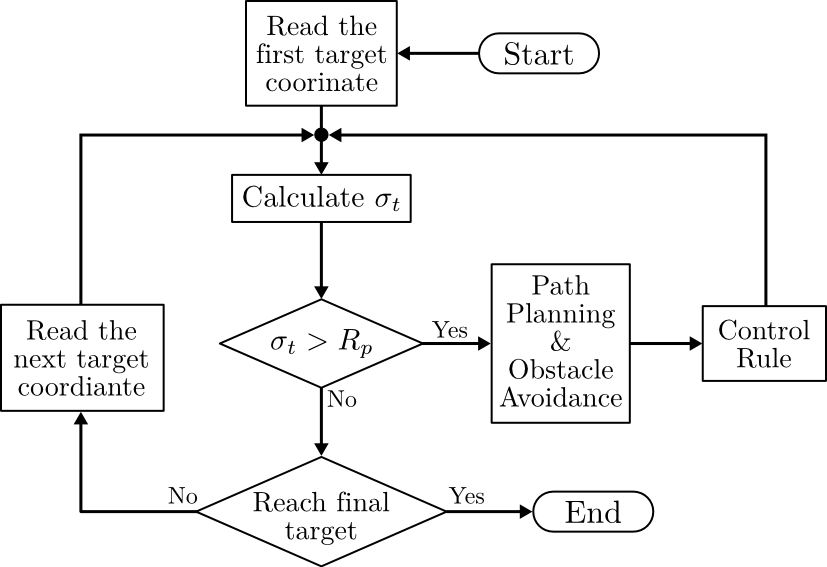
\includegraphics[width=0.8\textwidth]{figures/algorithm/navigation_flow}
	\caption{導航流程圖}
	\label{f:navigation_flow}
\end{figure}

\section{目標方向計算}
\label{sec:target}

\subsection{地理座標系統}
地理座標系統(Geographic Coordinate System)是用來表示地球上某個位置的座標系統,
這些座標系統可分為兩類:ECI(Earth Centered Inertial)與ECEF(Earth Centered Earth Fixed),
兩者之原點皆位於地球質心,但前者之座標系統不隨地球自轉而轉動,
座標軸永遠指向固定的方向(相對於星星);而後者之座標軸固定於地球上。
前者一般使用於天文學,像是找尋衛星的軌道等;
後者則多用來表示物體於地球上的位置,如GPS即使用ECEF系統。
簡單的ECEF座標系統可以用三維卡式座標系來表示,其原點位於地球的質心,
XY平面與地球的赤道平面重合,X軸指向經度$0\,^{\circ}$,
Y軸則是指向東經$90\,^{\circ}$,如圖~\ref{f:ecef}所示。
\begin{figure}[h!]
	\centering
	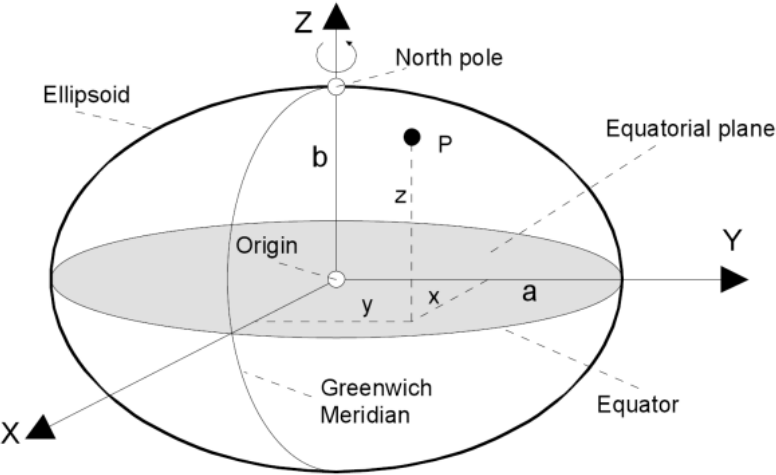
\includegraphics[width=12cm]{figures/algorithm/ECEF}
	\caption{ECEF座標系統}
	\caption*{來源:MTi-G Manual}
	\label{f:ecef}
\end{figure}

雖然能夠使用各種座標系統來表示位置,但一般最常使用的是ECEF橢球座標系(Ellipsoidal Coordinates),
使用緯度(Latitude)$\phi$、經度(Longitude)$\lambda$與高度(Altitude)$h$來表示三維空間中的點,
如圖~\ref{f:ellipsoid}所示,因為地球的形狀最接近橢球。
此處的橢球為一雙軸橢球(Biaxial Ellipsoid),為一橢圓以短軸為旋轉軸旋轉一圈後得到的表面。
\begin{figure}[h!]
	\centering
	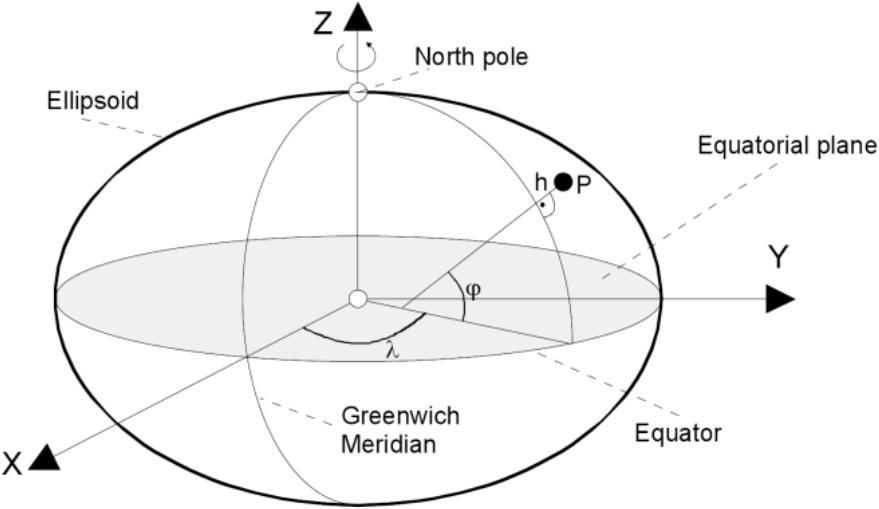
\includegraphics[width=12cm]{figures/algorithm/ellipsoid}
	\caption{橢球座標系}
	\caption*{來源:MTi-G Manual}
	\label{f:ellipsoid}
\end{figure}

橢球座標系會隨著定義的橢球不同而改變,而用來描述地球所定義的橢球就稱為大地基準(Datum)。
MTi-G位置感測器使用WGS84大地基準,而這個基準也是一般GPS所使用的標準座標系,
如圖~\ref{f:ecef}所示,而參數如表~\ref{t:wgs84}所示:
\begin{table}[h!]
	\centering
	\caption{WGS84大地基準參數}
	\label{t:wgs84}
	\begin{tabular}{ | l | c | }
		\hline
		長軸$a$ & $6378137m$ \\ \hline
		短軸$b$ & $6356752.3142m$ \\ \hline
		扁率$f$	& = $(a-b) / a = 1/298.257223563$ \\
		\hline
	\end{tabular}
\end{table}

另外要注意的是,在橢球上緯度的定義有三種:
地心(Geocentric)、修化(Reduced)與測地(Geodetic)緯度~\cite{Jekeli:2006:GRSinGeodesy}。
而最常見的緯度定義,包括WGS84,都是定義為測地緯度,
其定義為:若$P$為橢球座標系上的一點,則能夠找出一過該點的經度平面(Meridian Plane),
而測地緯度$\phi$為在此平面上,過$P$點且與該橢圓垂直的直線與長軸的夾角,
如圖~\ref{f:geodetic_latitude}所示。
\begin{figure}[h!]
	\centering
	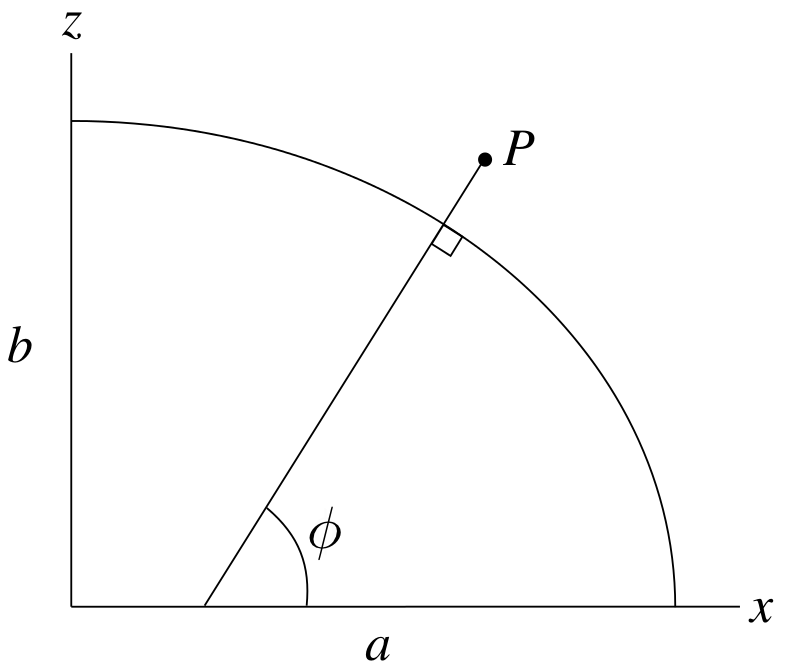
\includegraphics[width=6cm]{figures/algorithm/geodetic_latitude}
	\caption{測地緯度示意圖}
	\label{f:geodetic_latitude}
\end{figure}

\subsection{測地線}
測地線(Geodesic)在微分幾何學上有嚴謹的定義,
而在橢球曲面上可視為兩點之間的最短距離~\cite{Karney:2013:Algorithms_for_Geodesics}。
與其相關的問題可分為兩種:Direct與Inverse,
前者為給定起點$A(\phi_1,\lambda_1)$、方位角(azimuth)$\alpha_1$與距離$s_{12}$後計算終點位置$B$;
後者則是給定起點$A(\phi_1,\lambda_1)$與終點$B(\phi_2,\lambda_2)$,計算兩者之間的方位角$\alpha_1$與最短距離$s_{12}$,
如圖~\ref{f:geodesic}所示~\cite{Jekeli:2006:GRSinGeodesy}。
\begin{figure}[h!]
	\centering
	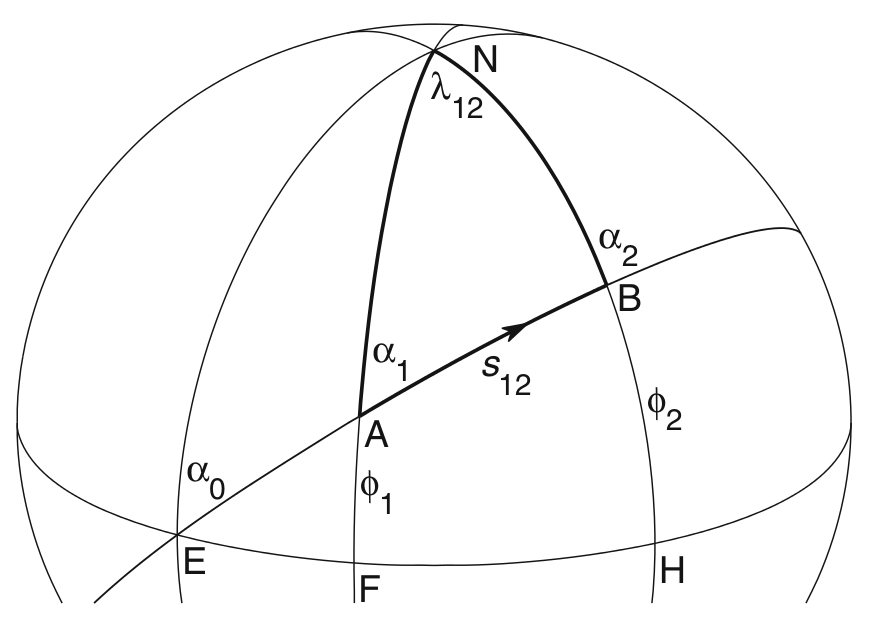
\includegraphics[width=6cm]{figures/algorithm/geodesic}
	\caption{測地線}
	\label{f:geodesic}
\end{figure}

本論文需要計算兩個位置之間(車輛與目標點)的方位角與距離,因此必須要解決上述的Inverse問題。
而測地線是微分幾何學上一個重要的研究對象,當曲面較為複雜時需要非常繁瑣的計算才能得到精準值,
詳細解法可參照~\cite{Karney:2013:Algorithms_for_Geodesics,Jekeli:2006:GRSinGeodesy}。
然而,由於電腦計算能力大幅增加,已經可以使用數值方法來解決Inverse問題:
假設$\alpha_1$為已知,因此利用已知的$\phi_1$、$\phi_2$及$\alpha_1$,
可以計算出相應的$\lambda_{12} = \lambda_2 - \lambda_1$,
因此便可利用牛頓法迭代$\alpha_1$以得到正確的$\lambda_{12}$,
此時的$\alpha_1$就是正確的解,同時也可計算出相應的$s_{12}$,
也就是車輛與目標點之間的距離$\sigma_t$~\cite{Karney:2013:Algorithms_for_Geodesics}。
本論文使用GeographicLib函式庫~\cite{website:GeographicLib}處理這個問題。

\subsection{區域座標系統}
區域切平面(Local Tangent Plane)為姿態量測系統的參考座標系,
其X軸指向正北方且與橢球相切,如圖~\ref{f:LTP}所示。
其量測的姿態角即為感測器座標系統相對於此座標系統之Cardan Angle,
即航空學上常用的Roll($\phi$)、Pitch($\theta$)與Yaw($\psi$)角。
\begin{figure}[h!]
	\centering
	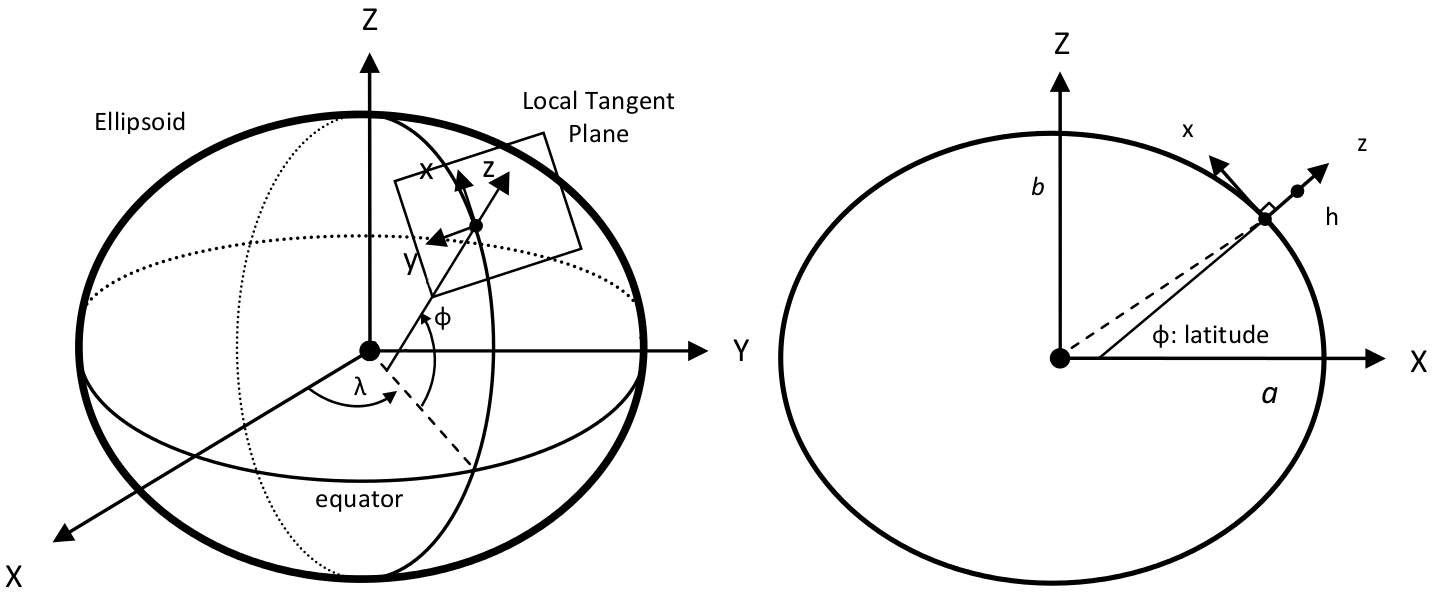
\includegraphics[width=\textwidth]{figures/algorithm/LTP}
	\caption{區域切平面示意圖}
	\caption*{來源:MTi-G Manual}
	\label{f:LTP}
\end{figure}

上一節所述之方位角$\alpha_1$為使用地理座標系統$\mathbf{G}$,相對於北方順時針方向所量測的角度;
Yaw角度$\psi$為使用區域座標系統$\mathbf{L}$,相對於北方逆時針方向量測之角度。
因此,目標方向$\Theta_t$於區域座標系統$\mathbf{L}$,相對於車輛之角度可依下式計算:
\begin{equation}
	[\Theta_t]_{\mathbf{L}} = -[\alpha_1]_{\mathbf{G}} - [\psi]_{\mathbf{L}}
\end{equation}
若$\Theta_t$為負值代表目標在車輛右側,若為正值則於位車輛左側,如圖~\ref{f:target_angle}所示。
\begin{figure}[h!]
	\centering
	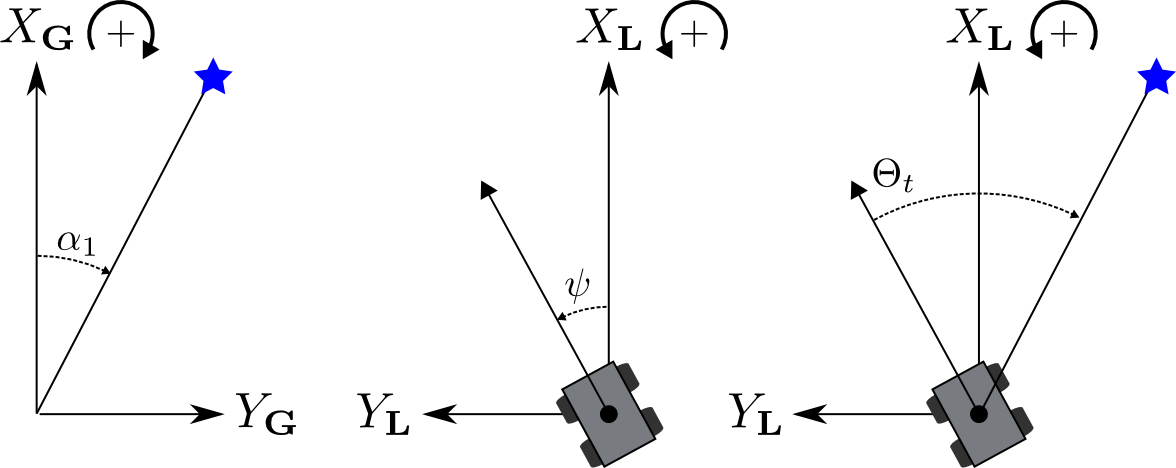
\includegraphics[width=\textwidth]{figures/algorithm/TargetAngle}
	\caption{目標方向相對於車輛之角度}
	\label{f:target_angle}
\end{figure}

\section{避障演算法}
\label{sec:vfhplus}

\subsection{常見演算法介紹}

\subsubsection{Artificial Potential Field}
Artificial Potential Field~\cite{Khatib:1985:APF}
使用環境資訊建立一虛擬力場,讓障礙物對機器人施加排斥力,
目標點則對其施加吸引力,兩者之合力即為機器人需要前進的方向。
藉由已知的地圖或是感測器所得到的資訊,能夠計算出一位能場$U(x,y)$,
其中障礙物具有較高的位能,而目標點具有較低的位能,
如圖~\ref{f:potential_field}所示。
接著對這個位能場做梯度運算,即可得到一虛擬力場$F(x,y)$:
\begin{equation}
	F(x,y) = -\nabla U(x,y)
\end{equation}
利用此虛擬力場,便能夠計算機器人在每個位置所需要的導航方向, 
指引機器人遠離障礙物並接近目標點。
\begin{figure}[h!]
	\centering
	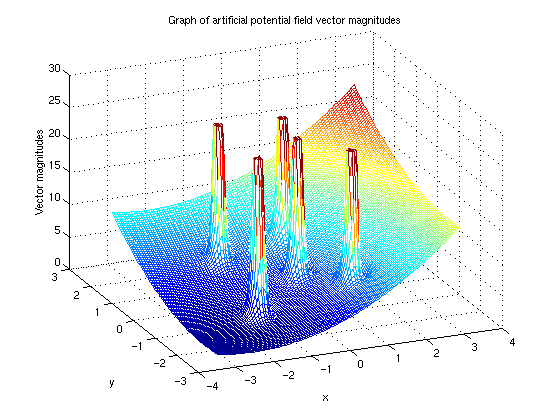
\includegraphics[width=10cm]{figures/algorithm/demo_apf_whitebg}
	\caption{位能場}
	\caption*{來源:people.csail.mit.edu}
	\label{f:potential_field}
\end{figure}

此演算法不只能夠做障礙物迴避,只要有地圖資訊也同時具有全域路徑規劃的能力,而且計算效率高。
然而此演算法假設機器人為單一質點,忽略機器人的動態拘束(最大加速度、機構拘束等)及幾何尺寸,
且於狹窄的空間中表現較差。

\subsubsection{Vector Field Histogram}
Vector Field Histogram(VFH)~\cite{Borenstein:1991:VFH}
將環境資訊以極座標直方圖(Polar Histogram)$D$的方式表示,橫軸為障礙之角度$\theta$,縱軸為其距離$d$,
接著找出可供機器人通過的空間,並計算其相對應的轉向角度,如圖~\ref{f:vfh}所示。
\begin{figure}[h!]
	\centering
	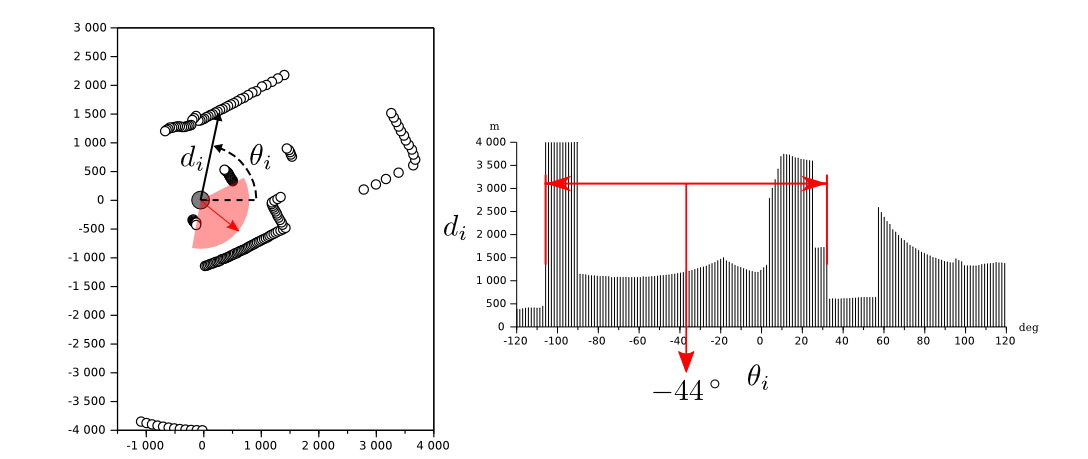
\includegraphics[width=\textwidth]{figures/algorithm/VFHTotal.png}
	\caption{極座標直方圖}
	\label{f:vfh}
\end{figure}

經過此計算後可能會出現多個可通過的候選轉向角度$\alpha_n$,此時可以使用成本函數(Cost Function)$G$
來計算每個轉向角度所要花費的「成本」:
\begin{equation}
	G = \mu_1 \delta_1 + \mu_2 \delta_2 + \mu_3 \delta_3
\end{equation}
其中$\delta_1$為目標方向與$\alpha_n$的差異;$\delta_2$為目前車輛方位角與$\alpha_n$的差異;
$\delta_3$為前一次計算得到的轉向角度與$\alpha_n$的差異,
而$\mu_1$、$\mu_2$與$\mu_3$代表的是各個差異值的權重系數。
$G$所計算出的值代表選擇該$\alpha_n$所需要耗費的成本,
藉由調整權重系數也能改變機器人導航時的趨勢。

VFH的極座標直方圖可直接套用光學雷達所得到的資訊,計算速度也相當快,
而且藉由成本函數也能夠調整機器人的導航特性。然而VFH並沒有考慮機器人的動態拘束與幾何尺寸,
而且\textbf{VFH所計算的轉向角度是由可通過的空間所決定的,並非目標方向}。
這是一個相當重要的特性,在狹窄的室內空間中這不會造成太大的影響,
然而在較為寬廣、障礙物較少的室外空間中,若光學雷達沒有偵測到障礙物,
此時演算法只會找到一個可通過的空間,以圖~\ref{f:vfh}來說就是從$-120\,^{\circ}$到$120\,^{\circ}$的範圍,
所以機器人只會朝著唯一的方向─正前方前進,直到偵測到障礙物,因此VFH並不適用於本論文。

\subsubsection{Curvature Velocity Method}
Curvature Velocity Method(CVM)~\cite{Simmons:1996:CVM}
考慮機器人的動態拘束,假設機器人的運動軌跡為曲率$c=\omega/\nu$的圓弧,
其中$\omega$代表機器人的旋轉速度(Rotational Velocity),$\nu$則是直線速度(Translational Velocity),
如圖~\ref{f:cvm_curvature}所示。因此,CVM使用速度空間$(\nu,\omega)$來做路徑規劃,而非卡式座標空間。
\begin{figure}
	\centering
	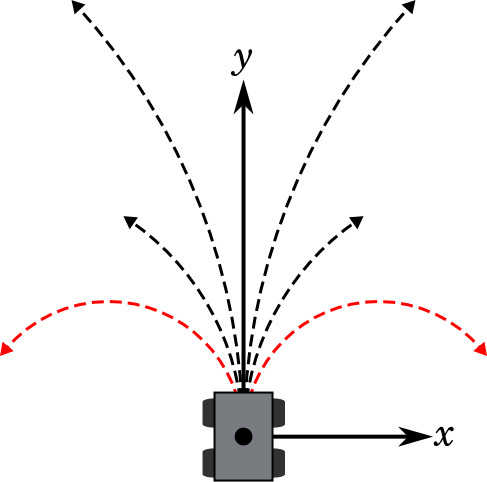
\includegraphics[width=8cm]{figures/algorithm/CVM1}
	\caption{CVM下的機器人運動軌跡}
	\label{f:cvm_curvature}
\end{figure}

為了將障礙物轉換至速度空間,設定一距離函數$D(c,OBS)$為沿著曲率$c$行走直到與障礙物集合$OBS$接觸的距離。
接著設定一最大行走距離$L$,表示機器人所能感測到的最大距離,此時距離函數將成為$D_{limit}$:
\begin{equation}
	D_{limit}(c,OBS) = min(L,D(c,OBS))
\end{equation}
為了計算方便,CVM將障礙物簡化為圓形,因此便能快速的將障礙物資訊轉換至速度空間。

CVM同樣使用一目標函數(Objective Function)$f$計算最佳的$\nu$與$\omega$:
\begin{equation}
	f(\nu,\omega) = \mu_1 \cdot speed(\nu) + \mu_2 \cdot dist(\nu,\omega) + \mu_3 \cdot head(\omega)
\end{equation}
其中:
\begin{align*}
	speed(\nu)	&= \nu / \nu_{max} \\ 
	dist(\nu,\omega)	&= D_{limit}({\omega \over \nu},OBS) / L \\
	head(\omega)	&= 1 - |\theta_{target} - \omega \cdot T_{c} | / \pi \\
\end{align*}
$\nu_{max}$為最大直線速度,$\theta_{target}$為目標方向,$T_c$為一時間常數。
此函數與先前的成本函數相反,產生最大值的$(\nu,\omega)$才是最佳值。

CVM藉由速度空間設定動態拘束,可設定最大速度與最大加速度來限制其運動狀態。
幾何拘束也可利用放大障礙物的尺寸來調整。然而過於簡化的障礙物是其限制,
而且必須具備速度感測器才能使用此演算法,因此不適用於本論文。

\subsubsection{Dynamic Window Approach}
Dynamic Window Approach(DW)~\cite{Thrun:1997:DW}
與CVM相同,假設機器人之運動軌跡為曲率$c=\omega/\nu$的圓弧,
利用最大直線速度與最大旋轉速度建立一速度空間,並將量測到的環境轉換至此空間中,
如圖~\ref{f:DW_cartesian}及~\ref{f:DW_velocity}所示。
\begin{figure}[h!]
	\centering
	\begin{subfigure}[t]{0.6\textwidth}
		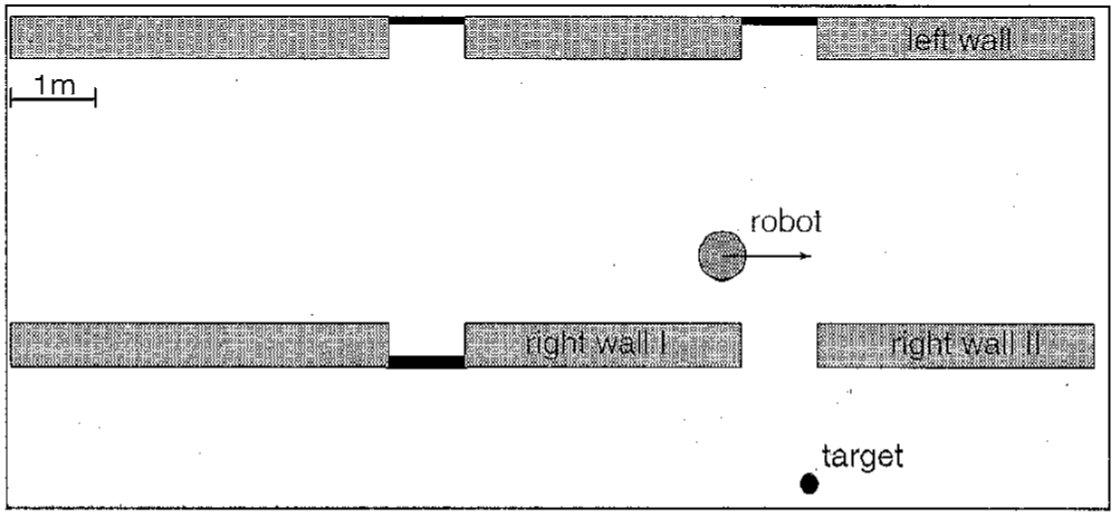
\includegraphics[width=\textwidth]{figures/algorithm/DW_cartesian}
		\caption{實際環境資訊}
		\label{f:DW_cartesian}
	\end{subfigure}
	\begin{subfigure}[t]{0.6\textwidth}
		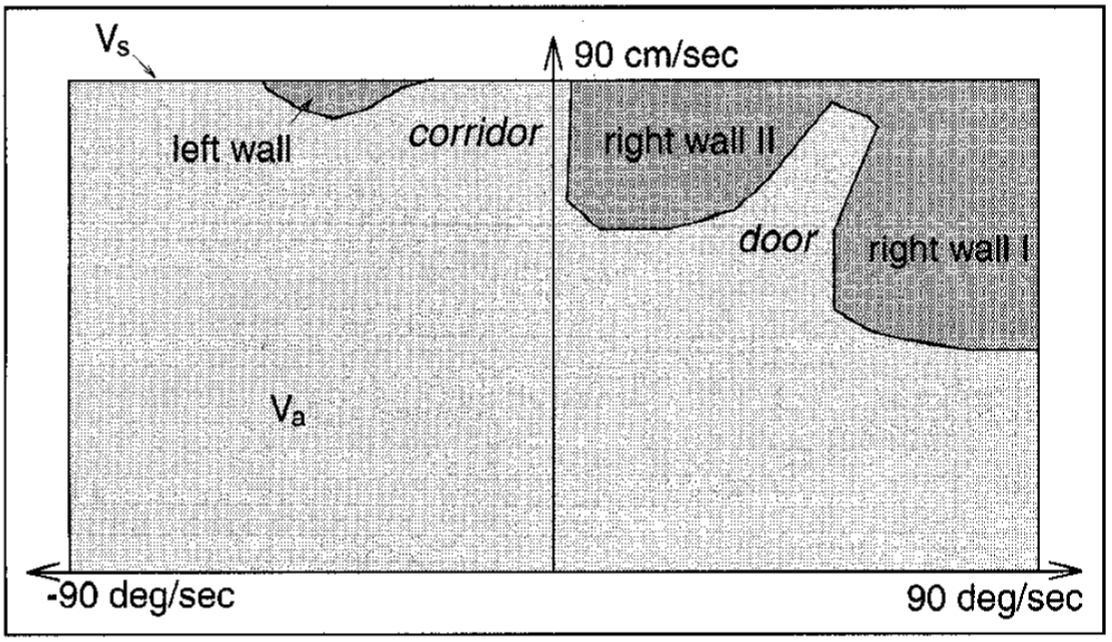
\includegraphics[width=\textwidth]{figures/algorithm/DW_velocity}
		\caption{速度空間中的環境資訊}
		\label{f:DW_velocity}
	\end{subfigure}
	\caption{環境資訊轉換}
	\caption*{來源:The Dynamic Window Approach to Collision Avoidance}
	\label{f:v_space}
\end{figure}
在圖~\ref{f:DW_velocity}中橫軸為旋轉速度,縱軸為直線速度;較暗的部分為被障礙物擋住的部分。

在速度空間中,根據機器人目前的速度以及最大加速度,可在速度空間中找出一動態視窗(Dynamic Window)$V_d$,
此視窗根據最大加速度限制了機器人所能達到的速度(視窗大小),
隨著機器人目前的速度不同此視窗的位置也會不斷改變,如圖~\ref{f:dynamic_window}所示。
\begin{figure}[h!]
	\centering
	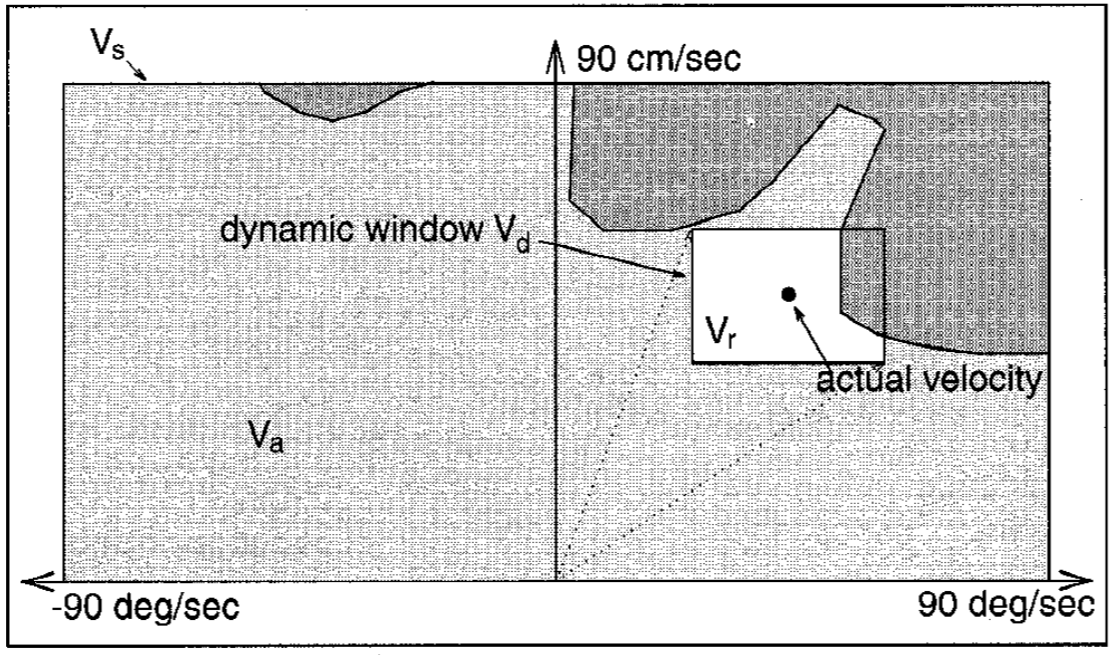
\includegraphics[width=10cm]{figures/algorithm/dynamic_window}
	\caption{動態視窗示意圖}
	\caption*{來源:The Dynamic Window Approach to Collision Avoidance}
	\label{f:dynamic_window}
\end{figure}
此視窗中的所有速度$(\nu,\omega)$代表了機器人所有可能達到的速度,而為了在此視窗中找出最佳解,
DW同樣使用目標函數來做最佳化。

藉由改變速度空間的形狀,DW能夠設定機器人的機構運動拘束,而動態視窗則考慮了機器人的動態拘束。
然而DW的計算較為複雜,且與CVM相同,都必須裝設速度感測器才能使用此演算法,因此並不適用於本論文。

\subsection{Vector Field Histogram Plus}
Vector Field Histogram Plus(VFH+)~\cite{Ulrich:1998:VFHPlus}
改進了許多VFH的缺點,將機器人的幾何限制和運動拘束也考慮在內。

原先的VFH+使用四個階段的計算逐一減少資訊量並找出轉向角度,而為了使用在光學雷達上,
本論文一樣使用四個階段的計算,但修改其計算方式與順序以便使用於光學雷達。
前面三個階段著重於根據機器人的拘束找出可通過的方向,最後一個階段則是計算最佳方向。

\subsubsection{階段一、極座標直方圖}
光學雷達所量測到的資訊可表示為$d_i$與$\theta_i$,$d_i$為第$i$個量測到的距離,
$\theta_i$則為$d_i$所對應的角度,如圖~\ref{f:LiDar_measurement}所示。
\begin{figure}[h!]
	\centering
	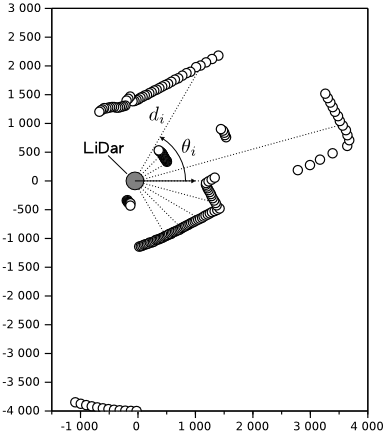
\includegraphics[width=8cm]{figures/algorithm/LiDar_measurement}
	\caption{光學雷達量測示意圖}
	\label{f:LiDar_measurement}
\end{figure}

與VFH相同,VFH+首先使用光學雷達所得到的資訊建立一極座標直方圖$P_i$:
\begin{equation}
	P_i = a - b\cdot d_i
\end{equation}
$a$與$b$皆為正值。藉由調整此處的$a$與$b$,使用者可調整VFH+所要偵測與計算的範圍。
圖~\ref{f:polar_histogram}為$a=1200$、$b=1$的設定下,
圖~\ref{f:LiDar_measurement}所量測到之環境產生的$d_i$與$P_i$示意圖。
\begin{figure}[h!]
	\centering
	\begin{subfigure}[b]{0.7\textwidth}
		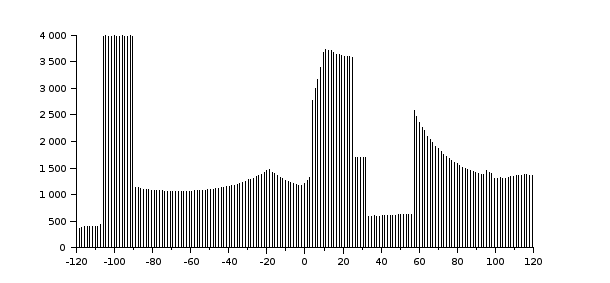
\includegraphics[width=\textwidth]{figures/algorithm/polar_histogram}
		\caption{$d_i$}
		\label{f:polar_histogram_original}
	\end{subfigure}
	\begin{subfigure}[b]{0.7\textwidth}
		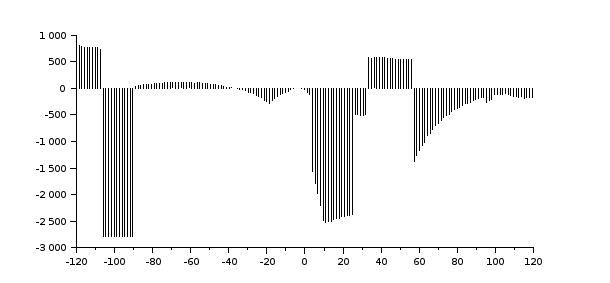
\includegraphics[width=\textwidth]{figures/algorithm/polar_histogram_modified}
		\caption{$P_i$}
		\label{f:polar_histogram_modified}
	\end{subfigure}
	\caption{極座標直方圖}
	\label{f:polar_histogram}
\end{figure}

\subsubsection{階段二、安全空間}
為了找出可供機器人通過的空間,VFH藉由一閾值$\tau$過濾出所有視為安全的距離,
而一段連續的安全距離就代表一個可通過的安全空間$V_j$,由一組邊界向量$(\mathbf{B_L},\mathbf{B_R})_j$定義,
定義其左邊界與右邊界的角度$\theta$與障礙物的距離$d$,視為機器人所能通過的方向:
\begin{align}
	\mathbf{B_L}	&= \begin{bmatrix}
				\theta_l & d_l
			   \end{bmatrix} \nonumber \\
	\mathbf{B_R}	&= \begin{bmatrix}
				\theta_r & d_r
			   \end{bmatrix}
	\label{e:boundary}
\end{align}
然而VFH只使用單一閾值可能會過濾出許多不連續的空間,
造成許多不必要的方向選擇出現,讓機器人在決定方向時產生左右搖擺的現象。
因此,VFH+使用兩個閾值$\tau_{max}$與$\tau_{min}$,
利用遲滯(Hysteresis)效果過濾掉這些不必要的空間,產生二元直方圖(Binary Histogram)$H_i$:
\begin{equation}
	H_i = 
	\begin{cases}
		1	& \textrm{if } P_i \geq \tau_{max} \\
		0	& \textrm{if } P_i \leq \tau_{min} \\
		H_{i-1}	& \textrm{otherwise}
	\end{cases}
\end{equation}
圖~\ref{f:binary_histogram_1}為使用單一門檻值$\tau=0$的過濾結果,圖~\ref{f:binary_histogram_2}
則為使用雙閾值$\tau_{min}=0,\tau_{max}=450$的過濾結果,值為$0$的區域代表可通過的安全空間。
圖中可看到單閾值過濾產生了四個區域,而雙閾值則只有二個。
\begin{figure}[h!]
	\centering
	\begin{subfigure}[b]{0.8\textwidth}
		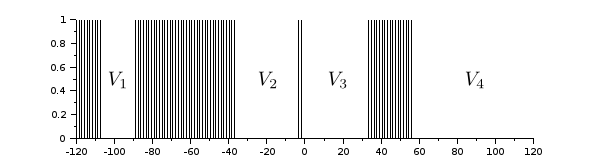
\includegraphics[width=\textwidth]{figures/algorithm/binary_histogram_1}
		\caption{單一閾值}
		\label{f:binary_histogram_1}
	\end{subfigure}
	\begin{subfigure}[b]{0.8\textwidth}
		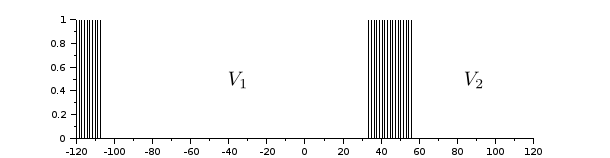
\includegraphics[width=\textwidth]{figures/algorithm/binary_histogram_2}
		\caption{雙閾值}
		\label{f:binary_histogram_2}
	\end{subfigure}
	\caption{過濾結果比較}
	\label{f:binary_histogram}
\end{figure}

原先的VFH忽略了機器人本身的幾何尺寸,而本論文使用縮小安全空間$V_j$邊界的方式來增加幾何拘束,
此時便可將機器人視為一質點。假設機器人之尺寸為半徑$w_s$的圓,則將$V_j$之邊界同樣縮小$w_s$後
便可將機器人視為一點,如圖~\ref{f:width}所示。
縮減後的安全空間$\hat{V_j} = (\hat{\mathbf{B_L}},\hat{\mathbf{B_R}})_j$可由式~\ref{e:width}計算:
\begin{align}
	\hat{\mathbf{B_L}}	&= \begin{bmatrix}
					\theta_l - \delta_l & d_l\cos\delta_l
				   \end{bmatrix},\delta_l = \arcsin({\frac{w_s}{d_l}}) \nonumber \\
	\hat{\mathbf{B_R}}	&= \begin{bmatrix}
					\theta_r + \delta_r & d_r\cos\delta_r
				   \end{bmatrix},\delta_r = \arcsin({\frac{w_s}{d_r}})
	\label{e:width}
\end{align}
\begin{figure}[h!]
	\centering
	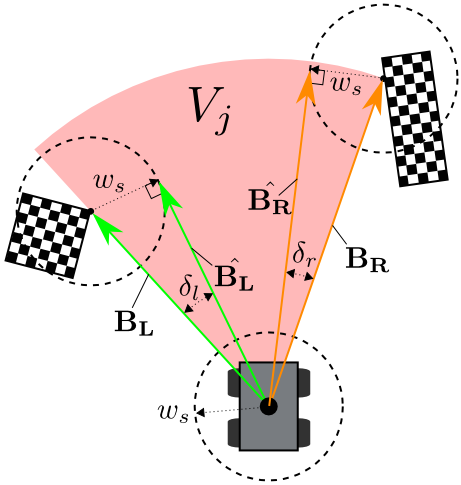
\includegraphics[width=0.5\textwidth]{figures/algorithm/width}
	\caption{邊界縮減}
	\label{f:width}
\end{figure}

\subsubsection{階段三、Blocked Directions}
VFH並沒有將機器人的動態拘束納入考慮,允許所有轉向角度的存在,然而這對某些轉向機構來說是不可能的。
因此VFH+使用機器人的最小迴轉半徑$R$與機器人尺寸$w_s$,計算出被障礙物所限制住的轉向角度$(\phi_l,\phi_r)$。
而原先的VFH+僅使用迴轉半徑$R$來計算,而本論文將機器人尺寸$w_s$加入計算,形成與迴轉半徑同心但半徑為$R+w_s$的圓,
如圖~\ref{f:block_directions}所示。
\begin{figure}
	\centering
	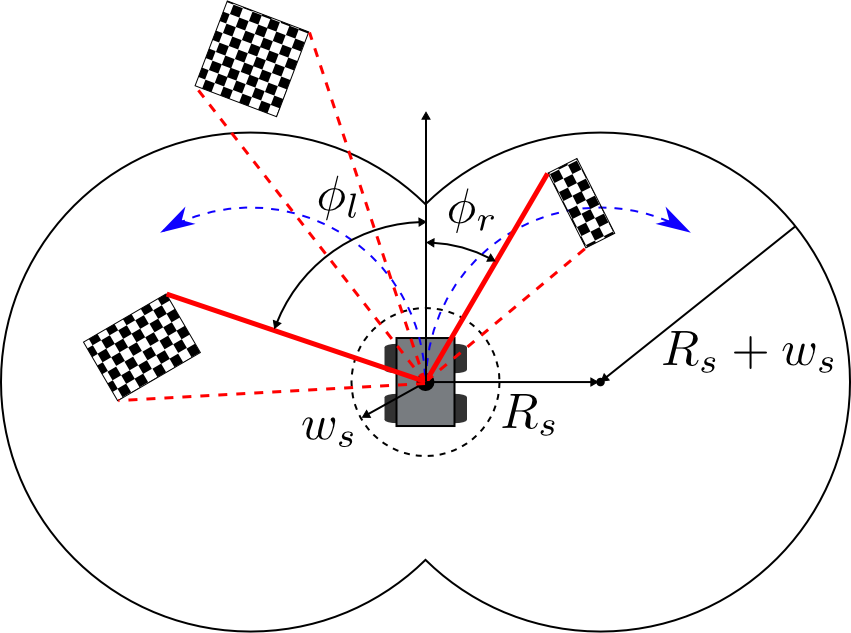
\includegraphics[width=0.8\textwidth]{figures/algorithm/blocked_directions}
	\caption{轉向角度限制}
	\label{f:block_directions}
\end{figure}

為了找出$(\phi_l,\phi_r)$,首先使用與光學雷達相同的$\theta_i$建立一偵測用的直方圖$D_i$,
偵測障礙物是否阻擋了轉向角度,如圖~\ref{f:detection_histogram}所示。其可由式~\ref{e:detection_histogram}計算。
\begin{figure}[h!]
	\centering
	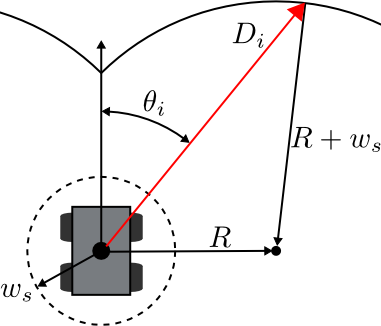
\includegraphics[width=0.5\textwidth]{figures/algorithm/detection_histogram}
	\caption{偵測直方圖示意圖}
	\label{f:detection_histogram}
\end{figure}
\begin{equation}
	D_i = |R\sin\theta_i| + \sqrt{R^2\sin^2\theta_i + w_s^2 + 2Rw_s}
	\label{e:detection_histogram}
\end{equation}
接著將光學雷達測得的$d_i$與$D_i$相減,所得到的直方圖稱為$M_i$
\begin{equation}
	M_i = d_i - D_i
\end{equation}
若$M_i$中對應於$\theta_i$之值小於$0$,則代表$\theta_i$有障礙物位於機器人之最小迴轉範圍內,
必須改變$(\phi_l,\phi_r)$限制轉向角度以避開障礙物。
環境與這些直方圖之間的轉換如圖~\ref{f:histogram_transform}所示。
\begin{figure}[h!]
	\centering
	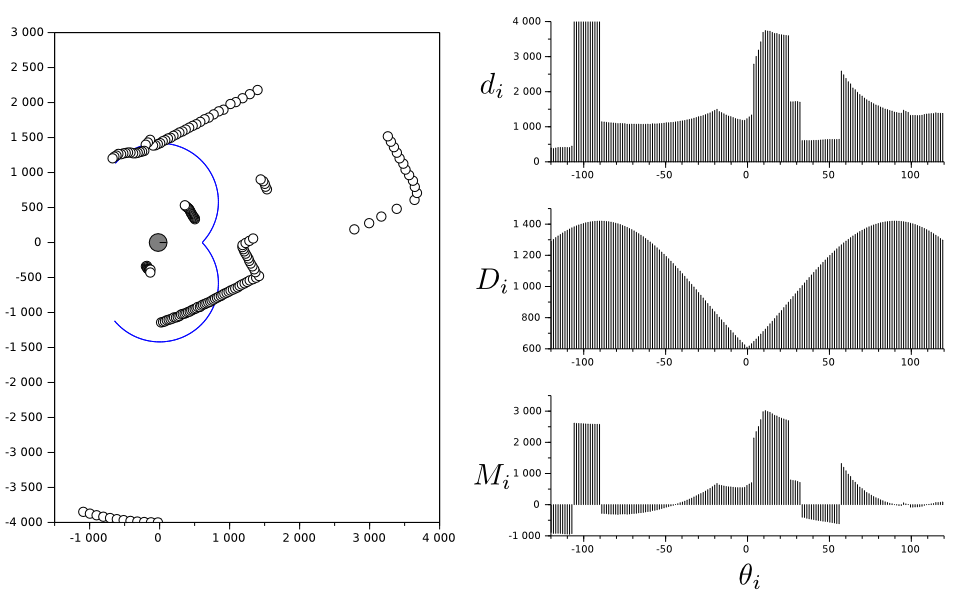
\includegraphics[width=\textwidth]{figures/algorithm/histogram_transform}
	\caption{直方圖轉換}
	\label{f:histogram_transform}
\end{figure}

利用$M_i$,$(\phi_l,\phi_r)$可以非常快速的被計算出來:
\begin{enumerate}
	\item{首先設$\phi_l = \pi$、$\phi_r = -\pi$}
	\item{對所有$i$,若$M_i < 0$:}
		\begin{enumerate}
			\item{若$\theta_i < 0$且$\theta_i > \phi_r$,則將$\phi_r$設為$\theta_i$}
			\item{若$\theta_i > 0$且$\theta_i < \phi_l$,則將$\phi_l$設為$\theta_i$}
		\end{enumerate}
\end{enumerate}

\subsubsection{階段四、Selection of Steering Direction}
根據安全空間$\hat{V_j}$的寬度,可以從每個$\hat{V_j}$中找到一個或多個候選方向$c$,
接著使用成本函數於這些候選方向中找出最佳解。
對於安全空間的寬度,本論文使用其邊界向量之間的角度差$\epsilon = \theta_l - \theta_r$做為判斷標準,
使用一角度閾值$\tau_a$與邊界縮減的情況將安全空間分為三種:交疊、狹窄與寬廣,如圖~\ref{f:epsilon_situation}所示。
\begin{figure}[h!]
	\centering
	\begin{subfigure}[t]{0.25\textwidth}
		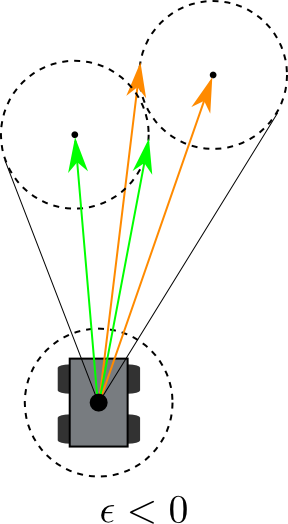
\includegraphics[width=\textwidth]{figures/algorithm/epsilon_situation_1}
		\caption{交疊}
		\label{f:epsilon_1}
	\end{subfigure}
	\begin{subfigure}[t]{0.3\textwidth}
		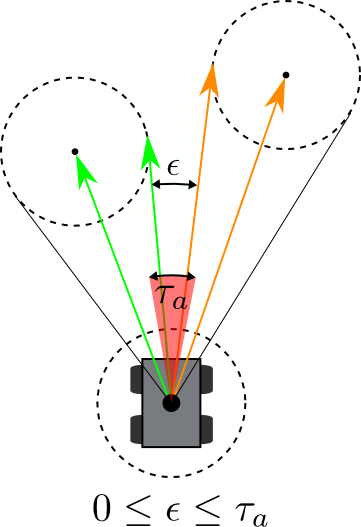
\includegraphics[width=\textwidth]{figures/algorithm/epsilon_situation_2}
		\caption{狹窄}
		\label{f:epsilon_2}
	\end{subfigure}
	\begin{subfigure}[t]{0.4\textwidth}
		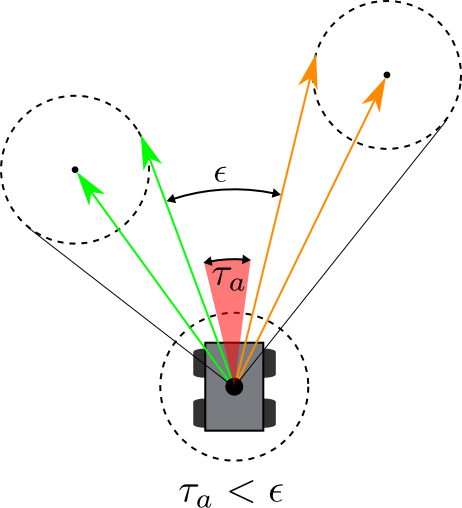
\includegraphics[width=\textwidth]{figures/algorithm/epsilon_situation_3}
		\caption{寬廣}
		\label{f:epsilon_3}
	\end{subfigure}
	\caption{邊界分類}
	\label{f:epsilon_situation}
\end{figure}

由於光學雷達在量測時是逆時針方向從$-120\,^{\circ}$掃描至$120\,^{\circ}$,在搜尋安全空間時也是同一方向,
因此每個安全空間的右邊界角度一定小於左邊界角度。因此,若是右邊界角度大於左邊界代表發生了邊界交疊,
此時該安全空間將會被捨棄,不會產生任何候選方向,如圖~\ref{f:epsilon_1}所示。

圖~\ref{f:epsilon_2}為狹窄($0 < \epsilon < \tau_a$)的安全空間,此時只有正中央的方向是唯一的候選方向:
\begin{equation}
	c_n = \frac{\theta_l + \theta_r}{2}
\end{equation}

圖~\ref{f:epsilon_3}則為寬廣($\epsilon > \tau_a$)的安全空間。
於此空間中候選角度有二個或三個,分別為兩邊界向量所對應的角度,以及當目標方向$\Theta_t$落在此範圍中,則$\Theta_t$也是候選角度之一。
\begin{align}
	c_r &= \theta_r \nonumber \\
	c_l &= \theta_l \nonumber \\
	c_T &= \Theta_t \text{ , if } \theta_l < \Theta_t < \theta_r 
\end{align}

最後使用一成本函數$G$於這些候選轉向角中找出最佳解:
\begin{equation}
	G(c) = \mu_1\cdot(|c - \Theta_t|) + \mu_2\cdot(|c|) + \mu_3\cdot(|c - c_{t-1}|)
	\label{e:cost_function}
\end{equation}
在式~\ref{e:cost_function}中,第一項$(|c - \Theta_t|)$代表候選方向與目標方向之間的差距。
差距越大表示該候選角會將機器人帶離目標方向,所以成本將會增加。

第二項$(|c|)$代表候選方向與目前車輛方向的差距。這些候選角都是以車身座標系做為參考,
所以車輛本身方位角相對於此座標系將永遠是$0$,而候選方向越大代表機器人將會偏離目前的方向越多,
進而增加成本。

第三項$(|c - c_{t-1}|)$則代表候選角與前一次選擇的轉向角之間的差距。
這個差距越大代表機器人的越容易偏離目前的航向,造成擺盪的現象。

$\mu_1,\mu_2,\mu_3$則是相對應的權重係數,藉由調整這三個係數之間的相對大小,
機器人的導航特性就能夠被調整,而於成本函數中產生最小值的候選方向即為最佳方向$c_t$。

\subsection{問題討論與補償}
\label{subsec:problem}
VFH+演算法在大部分的情況下都能夠成功找出正確的轉向角度以迴避障礙物,然而有兩個情況會導致計算錯誤,
以下將討論這兩種情況。

\subsubsection{無候選方向}
VFH+對機器人的轉向有許多的限制,因此有時會發生無候選方向的情況。
這種情況時常發生於狹窄的空間,同時前方已無路可走且機器人之機構限制無法迴轉離開時。
然而,有時是因為VFH+演算法的特性造成誤判,將可通過空間判定為無法通過,圖~\ref{f:no_way_to_go}即為一誤判的例子。
在圖~\ref{f:no_way_to_go_measured}中,藍色虛線為機器人的最小迴轉半徑,可看到右前方的確擁有足夠的空間供機器人通過,
然而此時VFH+會因為邊界交疊的關係將此安全空間捨棄,造成無候選方向的情形,進而讓導航停止。
\begin{figure}[h!]
	\centering
	\begin{subfigure}[t]{0.48\textwidth}
		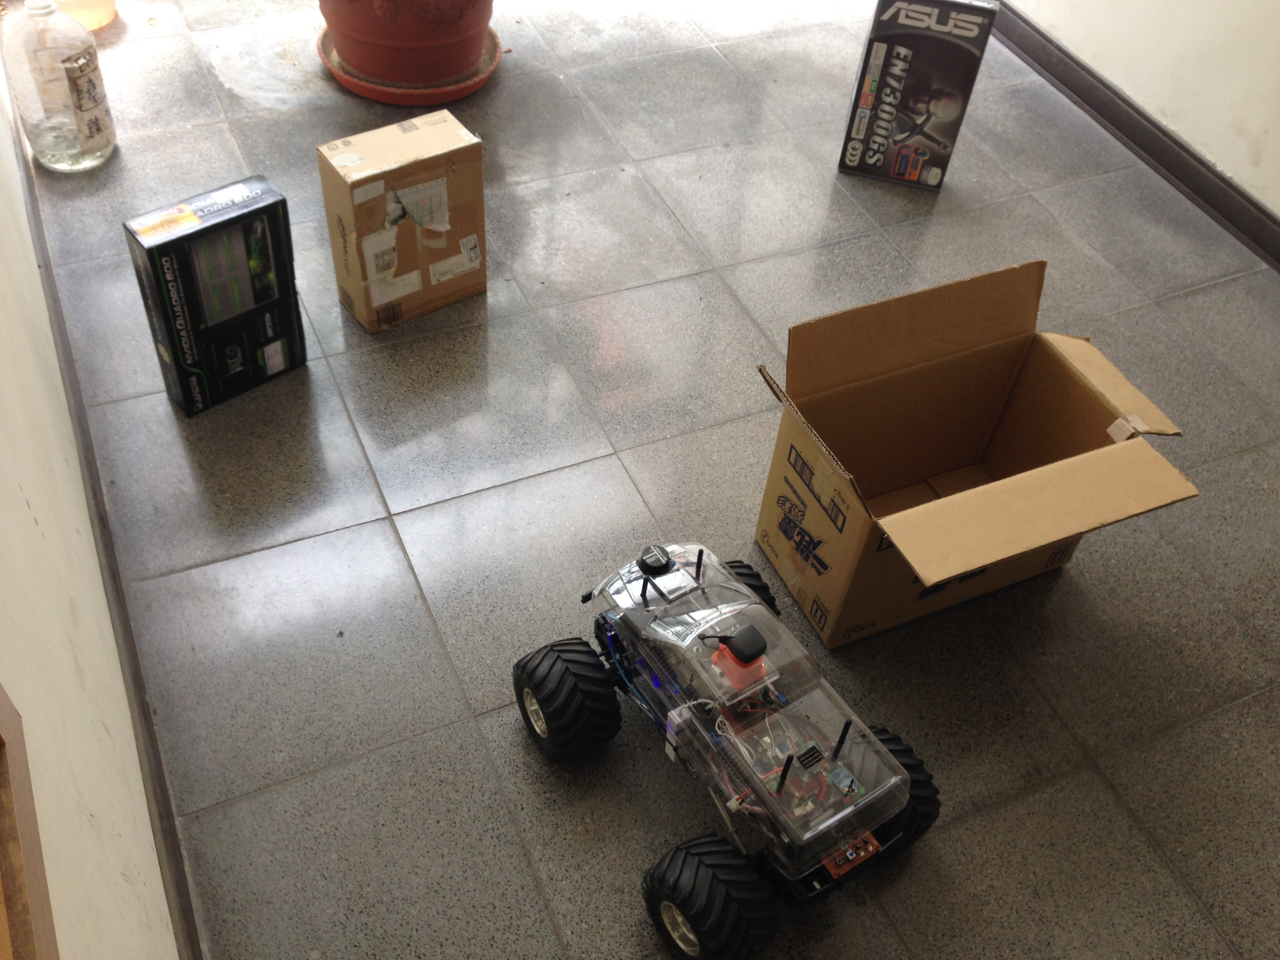
\includegraphics[width=\textwidth]{figures/algorithm/NoWayToGo_Real}
		\caption{實際情況}
		\label{f:no_way_to_go_real}
	\end{subfigure}
	\begin{subfigure}[t]{0.48\textwidth}
		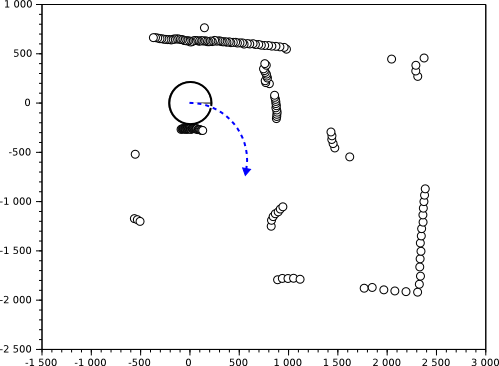
\includegraphics[width=\textwidth]{figures/algorithm/NoWayToGo}
		\caption{光學雷達量測結果}
		\label{f:no_way_to_go_measured}
	\end{subfigure}
	\caption{無候選轉向角之環境}
	\label{f:no_way_to_go}
\end{figure}
此問題將會使用速度控制與碰撞偵測補償,於~\ref{sec:speed_algorithm}節詳加介紹。

\subsubsection{安全空間邊界誤判}
為了將VFH+使用在光學雷達上,本論文使用安全空間取代了原始計算方法,以增加計算效率。
此方法在大部分情況下都能快速且有效的找出安全空間之邊界向量,然而在某些特殊情況下,
此方法會得到不正確的邊界向量,進而計算出錯誤的轉向角度,圖~\ref{f:wrong_boundary}即為一範例,
而依圖~\ref{f:wrong_boundary}之環境產生之各直方圖如圖~\ref{f:closest_histograms}所示。
\begin{figure}[h!]
	\centering
	\begin{subfigure}[t]{0.51\textwidth}
		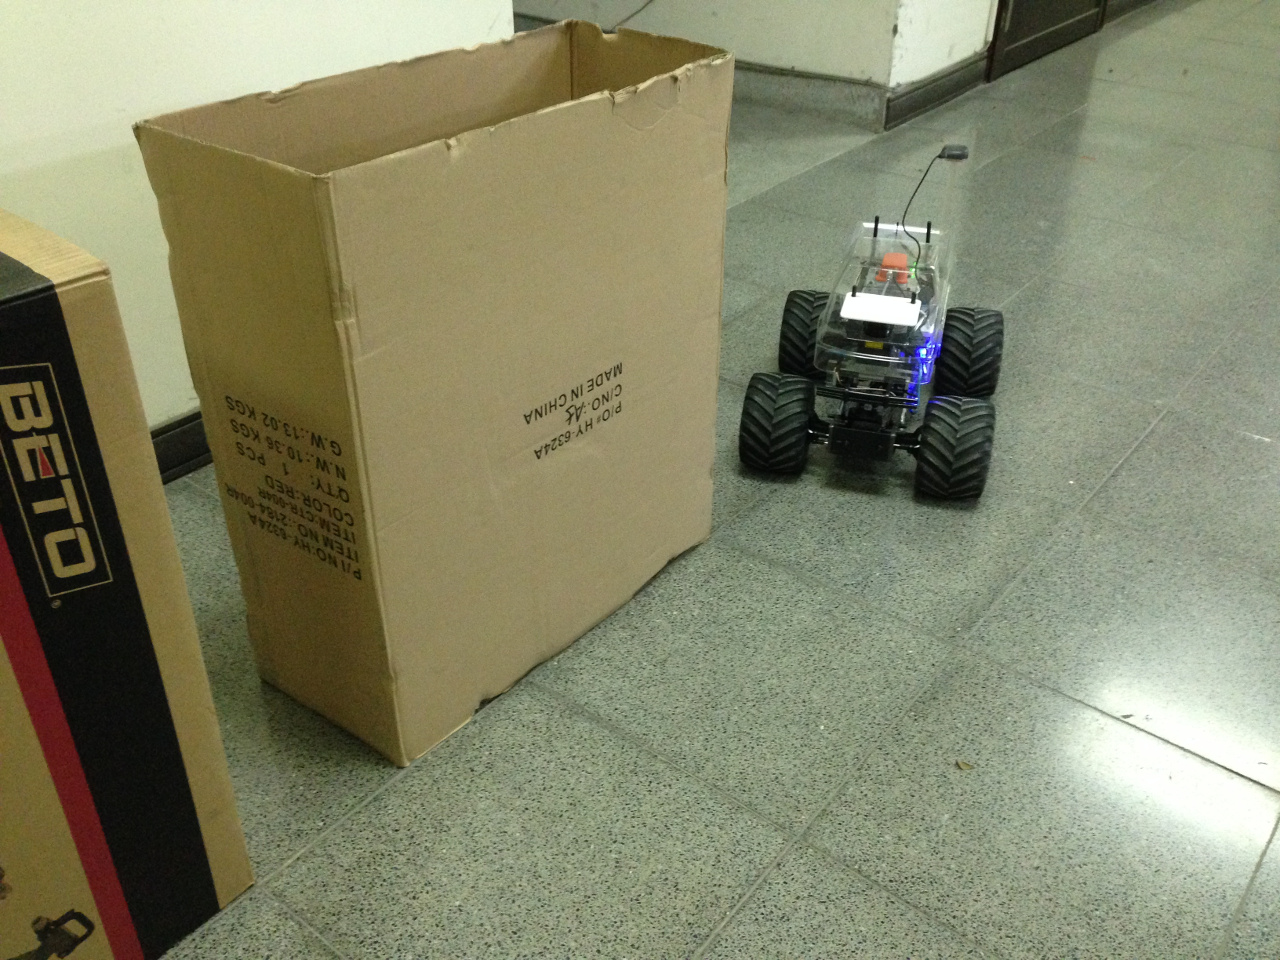
\includegraphics[width=\textwidth]{figures/algorithm/wrong_boundary_real}
		\caption{實際情況}
		\label{f:wrong_boundary_real}
	\end{subfigure}
	\begin{subfigure}[t]{0.45\textwidth}
		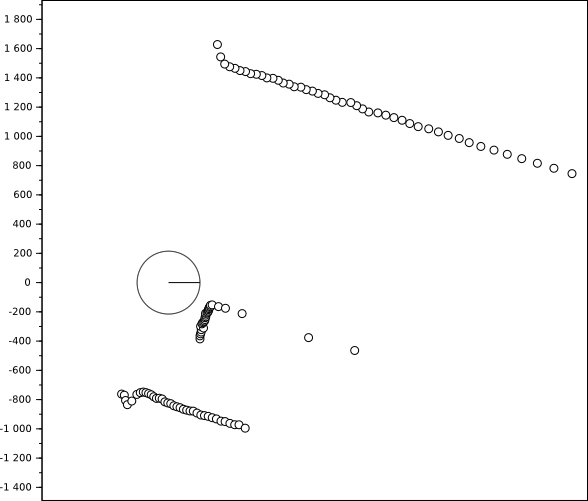
\includegraphics[width=\textwidth]{figures/algorithm/wrong_boundary}
		\caption{光學雷達量測結果}
		\label{f:wrong_boundary_m}
	\end{subfigure}
	\caption{安全空間邊界誤判之環境}
	\label{f:wrong_boundary}
\end{figure}
\begin{figure}
	\centering
	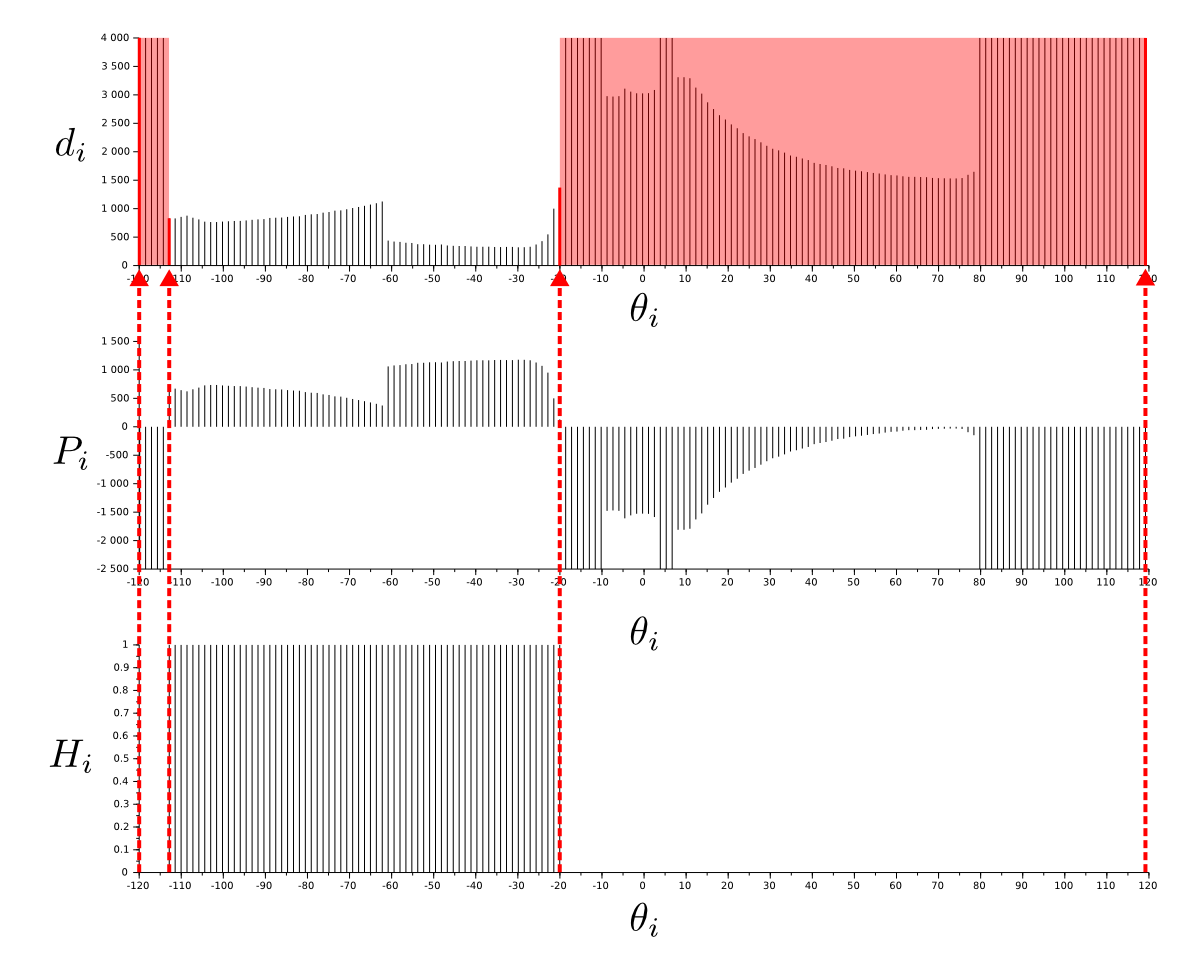
\includegraphics[width=0.92\textwidth]{figures/algorithm/closest_histograms}
	\caption{環境直方圖}
	\label{f:closest_histograms}
\end{figure}

由於找尋安全空間的方式是從二元直方圖$H_i$中找出連續為$0$的區域,
並根據此區域的邊界於$d_i$中找出相對應的邊界向量$(\mathbf{B_L},\mathbf{B_R})$,
因此邊界向量會是離該空間最近的兩個向量,如圖~\ref{f:closest_histograms}所示。
根據此計算方式,於圖~\ref{f:wrong_boundary}的環境下所找出的空間邊界與進行邊界縮減後的方向如圖~\ref{f:w_b_wrong_direction}所示。
而此時量測到的邊界會造成縮減角度不足,計算出錯誤的轉向角度,即為發生了邊界誤判。
\begin{figure}
	\centering
	\begin{subfigure}[t]{0.8\textwidth}
		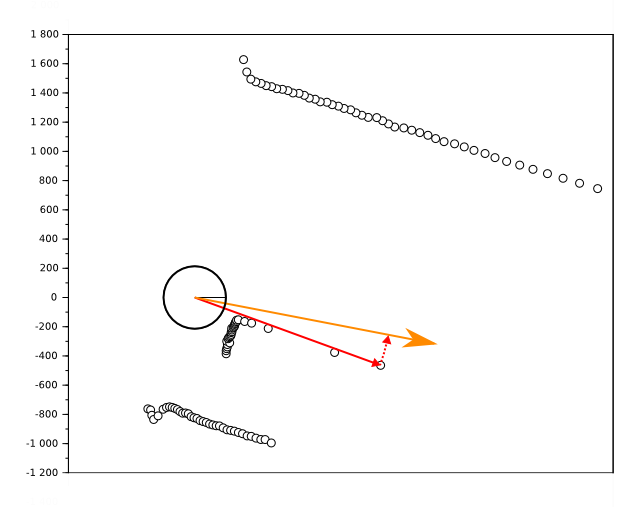
\includegraphics[width=\textwidth]{figures/algorithm/w_b_wrong_direction}
		\caption{計算後的邊界方向}
		\label{f:w_b_wrong_direction}
	\end{subfigure}
	\begin{subfigure}[t]{0.8\textwidth}
		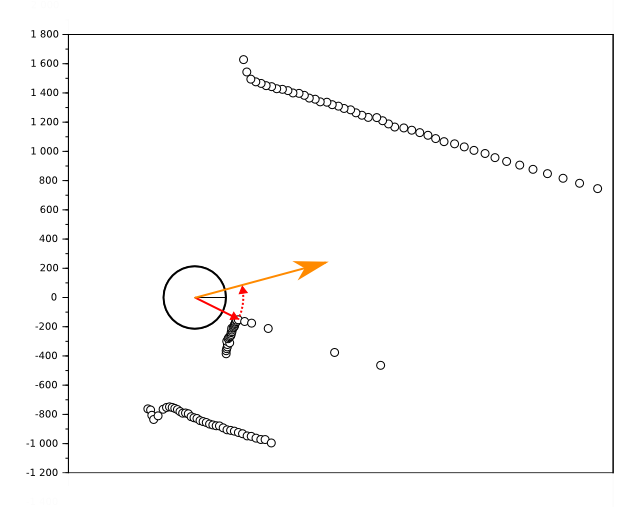
\includegraphics[width=\textwidth]{figures/algorithm/w_b_right_direction}
		\caption{實際之邊界方向}
		\label{f:w_b_right_direction}
	\end{subfigure}
	\caption{邊界縮減後之方向}
	\label{f:wrong_boundary_directions}
\end{figure}

由圖~\ref{f:wrong_boundary}可觀察到,真正的邊界應為障礙物之頂角,如圖~\ref{f:w_b_right_direction}所示。
因為距離較近,此邊界能夠提供機器人足夠的縮減角度,讓機器人能夠安全通過該空間。

為了解決此問題,可以對每一個量測值$d_i$與其角度$\theta_i$依前述的邊界縮減方式,計算所有量測值對機器人轉向角度的限制,如此便可找出真正的邊界向量。
然而此計算相當費時,而且對轉向角限制最大的通常是距離最近的障礙物,因此本論文僅計對距離機器人最近的量測值$d_{min}$與其角度$\theta_{min}$
計算邊界縮減值,找出其對機器人轉向角的限制範圍$(R_l,R_r)$,如圖~\ref{f:closest_boundary}所示。
若是邊界縮減後的安全空間之右邊界角度落在此範圍內,則將該邊界之角度設為$R_l$;
若縮減後的左邊界角度落在此範圍內,則將該邊界之角度設為$R_r$。如此,便可補償邊界誤判的問題,同時不致於降低計算效率。

\begin{figure}
	\centering
	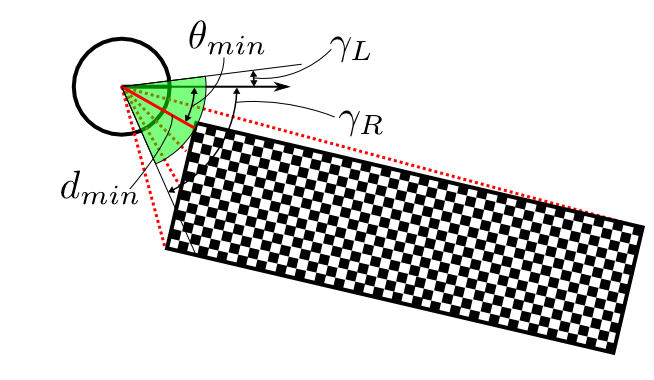
\includegraphics[width=0.9\textwidth]{figures/algorithm/closest_boundary}
	\caption{最近距離之邊界縮減}
	\label{f:closest_boundary}
\end{figure}

\section{速度演算法}
\label{sec:speed_algorithm}
\subsection{障礙物密度}
原先的VFH+使用障礙物密度函數$D$來計算機器人於該環境狀態下的速度,
而此函數可使用光學雷達的量測結果$d_i$與最大量測距離$d_{max}$計算:
\begin{equation}
	D(d_i) = 1 - \frac{1}{N}\sum_{i=1}^{N}{\frac{d_i}{d_{max}}}
\end{equation}
此函數所計算之值將會落在$0$與$1$之間,越接近$1$代表環境中的障礙物距離越近或數量較多(密度較高);
反之越接近$0$代表障礙物距離越遠或數量較少(密度較低)。因此,若設定機器人之最大速度$v_{max}$與最小速度$v_{min}$,
其速度$v$可依下式計算:
\begin{equation}
	v = v_{min} + (1-D(d_i)) \cdot (v_{max} - v_{min})
\end{equation}

雖然使用障礙物密度來計算速度是相當有效的方式,但此密度僅使用當時所處的環境進行計算,
並沒有將機器人當下的速度加入考慮。然而在進行路徑規劃時,若是機器人的速度過快,則機器人可能無法成功進行迴避,
來不及做出轉向反應,因此機器人當下的速度也是一個相當重要的因素。

\subsection{障礙物接近率}
由於本論文使用的實驗平台Yun-Trooper II並不具備速度感測器,無法直接獲得機器人的速度。
因此,本論文在原先的障礙物密度中增加一項障礙物接近率(Obstacle Approaching Rate)$\delta$,做為目前機器人速度的補償值。

障礙物接近率$\delta$的概念為,假設機器人位於一靜態環境中(障礙物的位置不隨時間而改變),
則若是量測到的環境變化相當大,代表機器人的速度較高;反之則代表速度較低。
而環境變化又以正前方的變化最為重要,因為這代表機器人接近正前方障礙物的速度,如圖~\ref{f:OAR}所示。
因此,設定一角度範圍,例如正前方左右各$20\,^{\circ}$,對所有位於此範圍內的光學雷達量測值$d_j$,
$\delta$可依下式計算:
\begin{equation}
	\delta = -\frac{1}{M}\sum_{j}\frac{(d_j)_t - (d_j)_{t-1}}{T}
\end{equation}
\begin{figure}
	\centering
	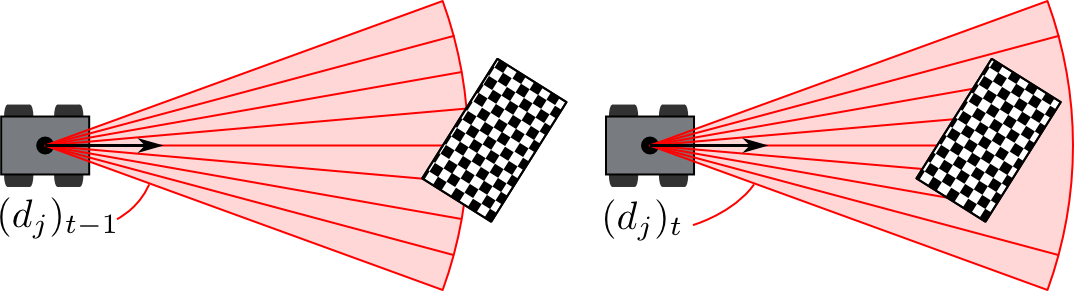
\includegraphics[width=0.9\textwidth]{figures/algorithm/obstacle_approaching_rate}
	\caption{障礙物接近率示意圖}
	\label{f:OAR}
\end{figure}
其中$(d_j)_t$代表當下的環境量測值;$(d_j)_{t-1}$代表上一次的環境量測值;
$T$代表兩次量測的時間間隔;$M$代表範圍內的量測值個數。

對路徑規劃來說,最重要的是以高速接近障礙物時能夠成功的減速,對加速的要求則相對較低。因此,在計算環境變化率時,
只將變化率$d_t - d_{t-1}$為負值(障礙物接近機器人)的方向納入計算,將變化率為正值的排除在外,得$\delta_a$:
\begin{equation}
	\delta_a = -\frac{1}{M}\sum_{j}\frac{\Delta((d_j)_t - (d_j)_{t-1})}{T}
\end{equation}
其中
\begin{equation*}
	\Delta(d) = 
	\begin{cases}
		d	& \textrm{if } d < 0 \\
		0	& \textrm{otherwise} \\
	\end{cases}
\end{equation*}

為了讓障礙物接近率與環境密度能夠一起計算,必須讓障礙物接近率的範圍落在$0$與$1$之間。
因此,將上式算出的$\delta_a$除以機器人的最大速度$v_{max}$便可得到落在$0$與$1$之間的障礙物接近率$\delta_n$:
\begin{equation}
	\delta_n = -\frac{1}{M \cdot v_{max}}\sum_{j}\frac{\Delta((d_j)_t - (d_j)_{t-1})}{T}
\end{equation}
$\delta_n$之值越接近$1$代表障礙物以較高的速度接近機器人;反之則代表障礙物以較低的速度接近。

最後,將環境變化率$\delta$列入考慮後,速度$v$可依下式計算:
\begin{equation}
	v = v_{min} + (1-(D(d_i)+\delta)) \cdot (v_{max} - v_{min})
	\label{e:speed_control}
\end{equation}

\subsection{碰撞偵測}
先前於~\ref{subsec:problem}中提到,因為避障演算法在某些情況下會發生誤判的情形,造成導航停止,
所以本論文在機器人的導航過程中不斷偵測碰撞是否即將發生,使用碰撞偵測做為導航停止與否的指標,而非轉向方向。

碰撞偵測可分為兩階段:
第一階段使用設定的機器人尺寸,偵測障礙物是否已經發生碰撞;
第二階段是偵測機器人的行進方向是否有障礙物存在,偵測碰撞是否即將發生。
只要其中一階段偵測到碰撞即代表碰撞發生,機器人將會停止前進。

\subsubsection{第一階段}
在設定機器人尺寸時,為了安全起見,通常會讓設定的尺寸比真實尺寸還大。
因此,第一階段的「已經發生碰撞」實際上代表的是,障礙物已經進入了設定的尺寸範圍內,而非真的發生了碰撞。
而由於在計算時已經將機器人的尺寸簡化為半徑為$w_s$的圓形,因此只要判斷光學雷達的量測值$d_i$是否小於$w_s$,
即可判定碰撞是否發生,如圖~\ref{f:collision_1stage}所示。
\begin{figure}[h!]
	\centering
	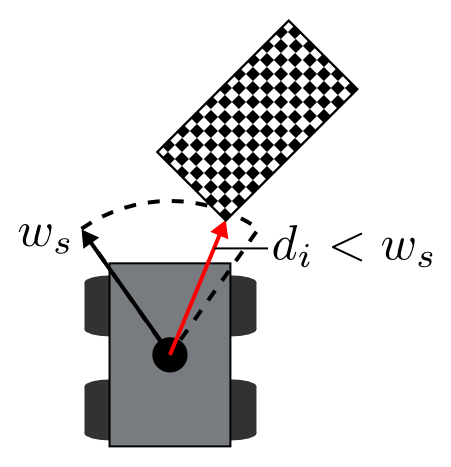
\includegraphics[width=0.5\textwidth]{figures/algorithm/collision_1stage}
	\caption{第一階段碰撞偵測示意圖}
	\label{f:collision_1stage}
\end{figure}

\subsubsection{第二階段}
若單純只使用機器人尺寸來偵測碰撞,在機器人速度較快時可能無法及時停止,讓機器人與障礙物實際發生碰撞,造成損壞。
因此,第二階段設定一距離$x$,利用車身尺寸$w_s$與轉向角度$c_t$建立一碰撞偵測範圍$\theta$,預先偵測行進路線上的障礙物,
以防止上述情況發生,如圖~\ref{f:collision_2stage}與式~\ref{e:collision_range}所示。
\begin{equation}
	\theta = \arctan{\frac{w_s}{x}}
	\label{e:collision_range}
\end{equation}
\begin{figure}[h!]
	\centering
	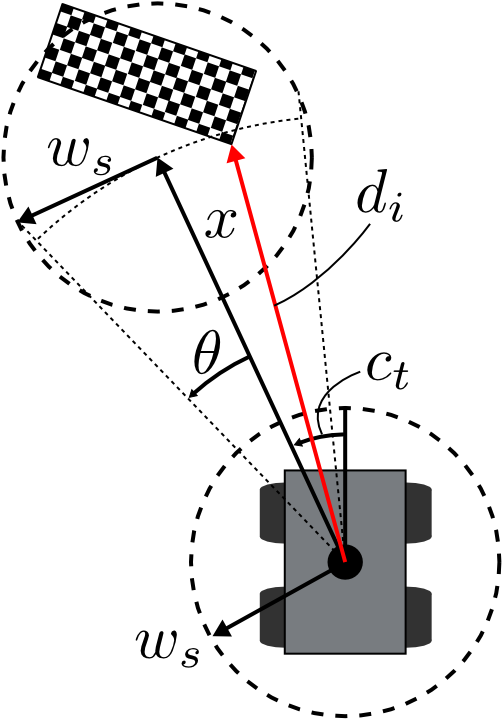
\includegraphics[width=0.45\textwidth]{figures/algorithm/collision_2stage}
	\caption{第二階段碰撞偵測示意圖}
	\label{f:collision_2stage}
\end{figure}

得到$\theta$後,可得到一角度範圍$\theta_r : c_t + \theta \leq \theta_r \leq c_t - \theta$。
在此角度範圍內的光學雷達量測值$d_i$若小於預先設定的距離$x$,如圖~\ref{f:collision_2stage}所示,
代表即將發生碰撞。

\section{控制法則}
綜合以上之演算法,機器人的轉向與速度控制法則使用虛擬碼表示如下:
\begin{center}
	\begin{algorithmic}[H]
		\If {$c_t \textrm{ is available}$}
			\State \textrm{steer} $\gets K \cdot c_t$
			\State \textrm{speed} $\gets v$
		\Else
			\State \textrm{steer} $\gets K \cdot c_{t-1}$
			\State \textrm{speed} $\gets v_{min}$
		\EndIf

		\If {\textrm{collision detected}}
			\State \textrm{speed} $\gets 0$
		\EndIf

		\State \textrm{setCommand\_Steer(steer)}
		\State \textrm{setCommand\_Speed(speed)}
	\end{algorithmic}
\end{center}
